\documentclass{beamer}

\usetheme{src/sintef}
\usefonttheme[onlymath]{serif}
\titlebackground*{beamerthemesrc/assets/background}
\setbeamertemplate{caption}[numbered]
%-------------add your packages here-------------
\usepackage[portuguese]{babel}
\usepackage{amsfonts,amsmath,oldgerm}
\usepackage{subfig}
\usepackage{graphicx}

\usepackage{tcolorbox}
\usepackage{adjustbox}
\usepackage{listings, listings-rust}

\usepackage{colortbl}
\usepackage{nicefrac, xfrac}

%-------------add your commands here-------------
\newcommand{\hrefcol}[2]{\textcolor{cyan}{\href{#1}{#2}}}
\newcommand{\testcolor}[1]{\colorbox{#1}{\textcolor{#1}{test}}~\texttt{#1}}

%-------------lst settings-----------------------

\colorlet{punct}{red!60!black}
\definecolor{background}{HTML}{EEEEEE}
\definecolor{delim}{RGB}{20,105,176}
\colorlet{numb}{magenta!60!black}
\definecolor{midgray}{gray}{.5}

\lstdefinelanguage{json}{
    basicstyle=\normalfont\ttfamily,
    stepnumber=1,
    numbersep=8pt,
    showstringspaces=false,
    breaklines=true,
    literate=
     *{0}{{{\color{numb}0}}}{1}
      {1}{{{\color{numb}1}}}{1}
      {2}{{{\color{numb}2}}}{1}
      {3}{{{\color{numb}3}}}{1}
      {4}{{{\color{numb}4}}}{1}
      {5}{{{\color{numb}5}}}{1}
      {6}{{{\color{numb}6}}}{1}
      {7}{{{\color{numb}7}}}{1}
      {8}{{{\color{numb}8}}}{1}
      {9}{{{\color{numb}9}}}{1}
      {:}{{{\color{punct}{:}}}}{1}
      {,}{{{\color{punct}{,}}}}{1}
      {\{}{{{\color{delim}{\{}}}}{1}
      {\}}{{{\color{delim}{\}}}}}{1}
      {[}{{{\color{delim}{[}}}}{1}
      {]}{{{\color{delim}{]}}}}{1},
}

\definecolor{template_brackes}{HTML}{0431FA}
\definecolor{template_keyword}{HTML}{859900}
\definecolor{template_magic_variable}{HTML}{268BD2}

\lstdefinelanguage{jinja2}{
    basicstyle=\normalfont\ttfamily,
    stepnumber=1,
    numbersep=8pt,
    showstringspaces=false,
    breaklines=true,
    literate=
     *{\{}{{{\color{template_brackes}\{}}}{1}
      {\}}{{{\color{template_brackes}\}}}}{1}
      {(}{{{\color{template_brackes}(}}}{1}
      {)}{{{\color{template_brackes})}}}{1}
      {\%}{{{\color{template_brackes}\%}}}{1}
      {loop}{{{\color{template_magic_variable}loop}}}{4}
      {recursive}{{{\color{template_keyword}recursive}}}{9}
      {if}{{{\color{template_keyword}if}}}{2}
      {else}{{{\color{template_keyword}else}}}{4}
      {for}{{{\color{template_keyword}for}}}{3}
      {endif}{{{\color{template_keyword}endif}}}{5}
      {endfor}{{{\color{template_keyword}endfor}}}{6}
      {set}{{{\color{template_keyword}set}}}{3}
      {not}{{{\color{template_keyword}not}}}{3}
      {[}{{{\color{delim}{[}}}}{1}
      {]}{{{\color{delim}{]}}}}{1},
}

%-------------title here--------------------
\title{Desenvolvimento de um software científico para a modelagem e simulação computacional}
\subtitle{Dissertação de Mestrado}
\course{Mestrado em Ciência da Computação}
\author{
    \hrefcol{mailto:dev@brenno.codes}{Brenno Lemos Melquíades dos Santos}
    \and \\
    \hrefcol{mailto:alexandre.pigozzo@ufsj.edu.br}{Orientador:  Prof. Alexandre B. Pigozzo}
}
\IDnumber{}

%--------------begin document--------------------
\begin{document}
\maketitle

\section{Introdução}
\begin{frame}{Introdução}
\end{frame}


\section{Referencial teórico}

\begin{frame}{Equações Diferenciais Ordinárias (EDOs)}
    \begin{itemize}
        \item Usadas para estudar o comportamento populacional ao longo do tempo;
        \item Diversas aplicações em várias áreas do conhecimento;
        \note[item]{Exemplos de uso de EDOs: medicina, neurociência, estudo do câncer.}
        \item Cada equação descreve a concentração de uma população diferente;
    \end{itemize}

    \begin{columns}
        \begin{column}{.4\textwidth}
            \begin{equation}
                \begin{array}{lr}
                    \frac{dN_1}{dt} = r_1.N_1(1 - W_{11}.N_1 - W_{21}.N_2)
                    \\
                    \\
                    \frac{dN_2}{dt} = r_2.N_2(1 - W_{22}.N_2 - W_{12}.N_1)
                \end{array}
            \end{equation}
        \end{column}

        \begin{column}{.6\textwidth}
            \begin{figure}
                \centering
                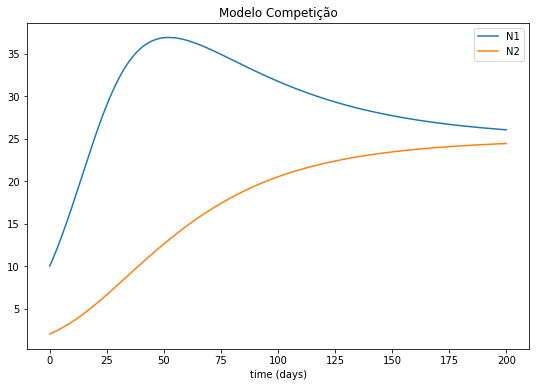
\includegraphics[height=.7\textheight]{beamerthemesrc/images/ode}
            \end{figure}
        \end{column}
    \end{columns}
\end{frame}

\begin{frame}{EDO — Modelo Predador-Presa}
    Um modelo clássico da literatura é o modelo Predador-Presa. Este modelo descreve o comportamento de duas populações, $H$ e $P$, que possuem uma uma relação de predação entre si. 

    \begin{columns}
        \begin{column}{.3\textwidth}
            \begin{equation}\label{eq:predadorpresa}
                \begin{array}{lr}
                    \frac{dH}{dt} = r.H - a.H.P
                    \\
                    \\
                    \frac{dP}{dt} = b.H.P - m.P
                \end{array}
            \end{equation}
        \end{column}
        \begin{column}{.6\textwidth}
            Na equação, temos que
            \[
            \begin{array}{lr}
                H & \text{Presa}\\
                P & \text{Predador}\\
                r & \text{Taxa de reprodução da presa}\\
                m & \text{Taxa de mortalidade dos predadores}\\
                a & \text{Taxa de predação}\\
                b & \text{Taxa de reprodução dos predadores}\\
                \end{array}.
            \]
        \end{column}
    \end{columns}

    \note[item]{
        Neste modelo, temos os seguintes processos sendo modelados: 
        \begin{itemize}
            \item Reprodução das presas ($r.H$);
            \item Predação ($a.H.P$);
            \item Reprodução dos predadores ($b.H.P$);
            \item Morte dos predadores ($m.P$). 
        \end{itemize}
    }
    \note[item]{
        Termos de replicação, predação e morte como os vistos neste modelo são muito comuns. Estes termos são construídos com base no princípio da Lei de Ação de Massas, que diz que ``O número de interações entre duas partículas depende da concentração de ambas.''
    }
\end{frame}

\begin{frame}{Programação visual}
    \begin{itemize}
        \item É uma maneira do usuário programar a máquina por meio de elementos gráficos que abstraem instruções do computador.
        \item Os elementos podem representar múltiplas operações por vez, com o objetivo de facilitar a programação.
        \item Exemplos: GRAIL, Scratch, Logisim, Blender. 
        \note[item]{A linguagem GRAIL foi desenvolvida junto a uma tela sensível ao toque e uma \textit{stylus}}
        \item Um exemplo comum de aplicação envolve editores baseados em nós, que representam operações complexas de forma natural, combinando um conjunto de entradas para gerar uma ou mais saídas.
    \end{itemize}
\end{frame}

\begin{frame}{Geração de código}
    \begin{itemize}
        \item Recebe como entrada uma Representação Intermediária (RI) e gera como saída um código na linguagem alvo (por exemplo, Python).
        \item Aplicações da RI: 
        \begin{itemize}
            \item Separar o \textit{front-end} do \textit{back-end};
            \item Permitir que sejam realizadas otimizações independente de máquina ou otimizações independente da linguagem alvo; 
            \item Facilitar a tradução e geração do código alvo.
        \end{itemize}
        \item Exemplo: LLVM IR, usada originalmente para compilar códigos em C/C++ pelo Clang, e agora também usada na compilação de códigos em Rust.
    \end{itemize}    
\end{frame}

\begin{frame}{Geração de código baseada em \textit{templates}}
    \begin{itemize}
        \item Um \textit{template} é um esqueleto (uma estrutura) que serve de referência para todo o processo de geração de código.
        \item Em sua essência, \textit{templates} são arquivos com marcadores especiais que podem ser substituídos por outros valores dinamicamente.
        \item A presença de estruturas de controle de fluxo como condicionais e laços de repetição permitem a escrita de \textit{templates} legíveis e de fácil manutenção.
    \end{itemize}
\end{frame}

\begin{frame}[fragile]{Geração de código baseada em \textit{templates}}
    \begin{minted}{python}
    def system(t: np.float64, y: np.ndarray, *constants) -> np.ndarray:
        
            {{- arg.name }},  = y

        
        
            {{- arg.name }},  = constants
        

        
        
        d{{ pop.name }}_dt = {{ display_composite(comp) }}
        

        # ...
    \end{minted}
\end{frame}

% \begin{frame}{Ensino-aprendizagem de Modelagem Computacional}
%     \begin{figure}[h]
%         \centering
%         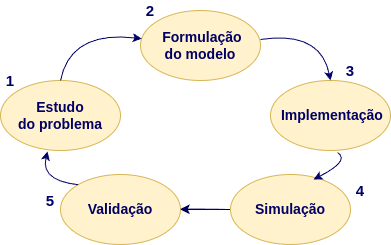
\includegraphics[scale=0.5]{contents/imgs/ciclo-modelagem.png} 
%         \caption{Visão geral do ciclo da modelagem.}
%         \label{fig:ciclo-modelagem}
%     \end{figure}
% \end{frame}


\section{Software para modelagem e simulação}
\begin{frame}{Visão geral do software}
    \begin{itemize}
        \item O software desenvolvido apresenta uma GUI contendo um editor baseado em nós.
        \item Os nós representam partes das equações, como parâmetros, populações e expressões
    \end{itemize}

    \begin{figure}
        \centering
        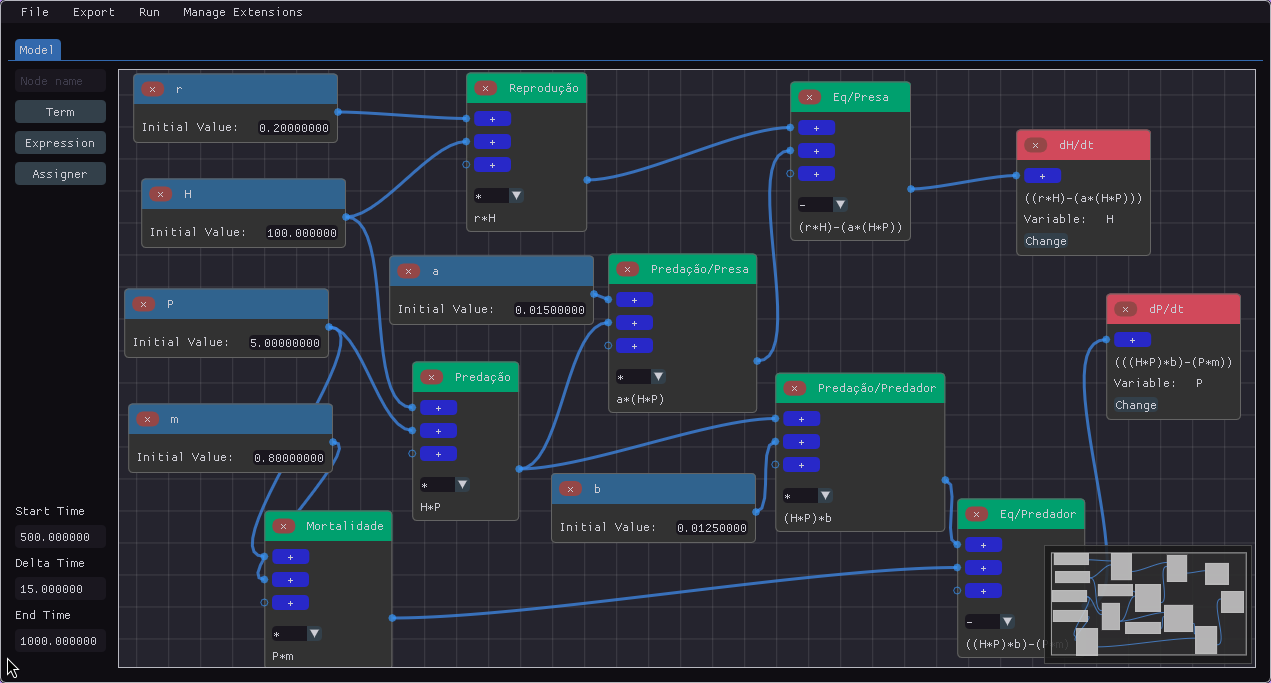
\includegraphics[width=0.75\textwidth]{contents/imgs/ode-designer/predador-presa-fit.png}
    \end{figure}
\end{frame}

\begin{frame}{Visão geral do software}
    \begin{columns}
        \begin{column}{.5\textwidth}
            Após construído o modelo, o usuário poderá simulá-lo diretamente pela GUI, exportar um PDF dos resultados, ou exportar um código de Python equivalente para o modelo desenhado
            \begin{figure}
                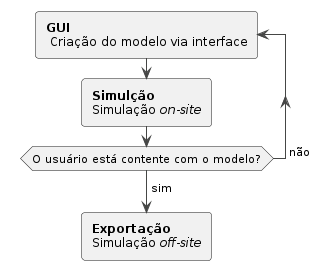
\includegraphics[width=.82\textwidth]{contents/imgs/fluxograma-exp.png}
            \end{figure}
        \end{column}
        \begin{column}{.5\textwidth}
            \begin{figure}
                \centering
                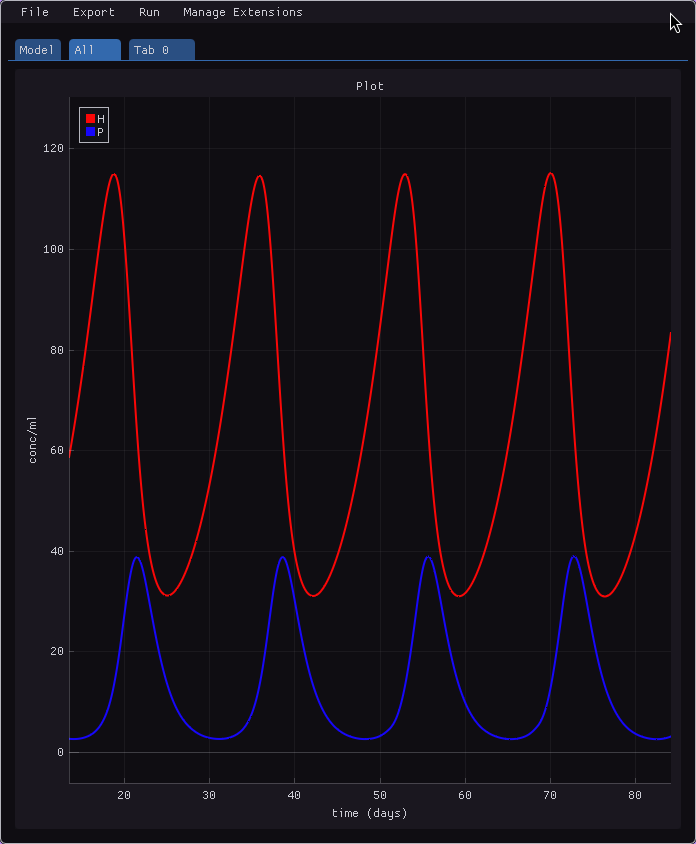
\includegraphics[width=.82\textwidth]{contents/imgs/ode-designer/grafico-thin.png}
            \end{figure}
        \end{column}
    \end{columns}
\end{frame}

\begin{frame}{Representação visual}
    \begin{table}
        \begin{center}
        \begin{tabular}{ m{0.12\textwidth}m{0.35\textwidth}m{0.4\textwidth} }
            \toprule
            Tipo de nó & Usado para representar & Exemplo \\
            \midrule
            Termo & Variáveis, parâmetros e constantes. & $H$, $P$, $a$, $b$, $r$, $m$ \\
            Expressão & Expressões matemáticas que compõem as equações. & \(r.H\), \(a.H.P\), \(r.H - a.H.P\);\\
            Equação & O lado direito de uma EDO. & \(dH/dt = ...\) \\
            \bottomrule
        \end{tabular}
        \end{center}
    \end{table}
    \begin{figure}
        \centering
        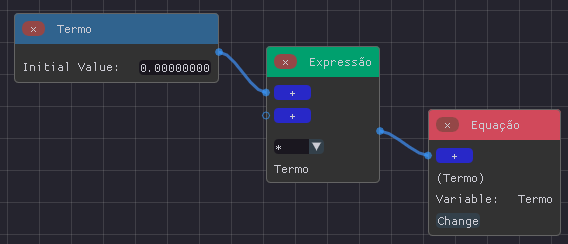
\includegraphics[width=.6\textwidth]{contents/imgs/ode-designer/tipos-nos-slim.png}
    \end{figure}
\end{frame}

% \begin{frame}{Árvore de expressões}

% \end{frame}

% \begin{frame}{Representação intermediária}

% \end{frame}

% \begin{frame}{Fluxograma de uso simplificado}
%     \begin{figure}
%         \centering
%         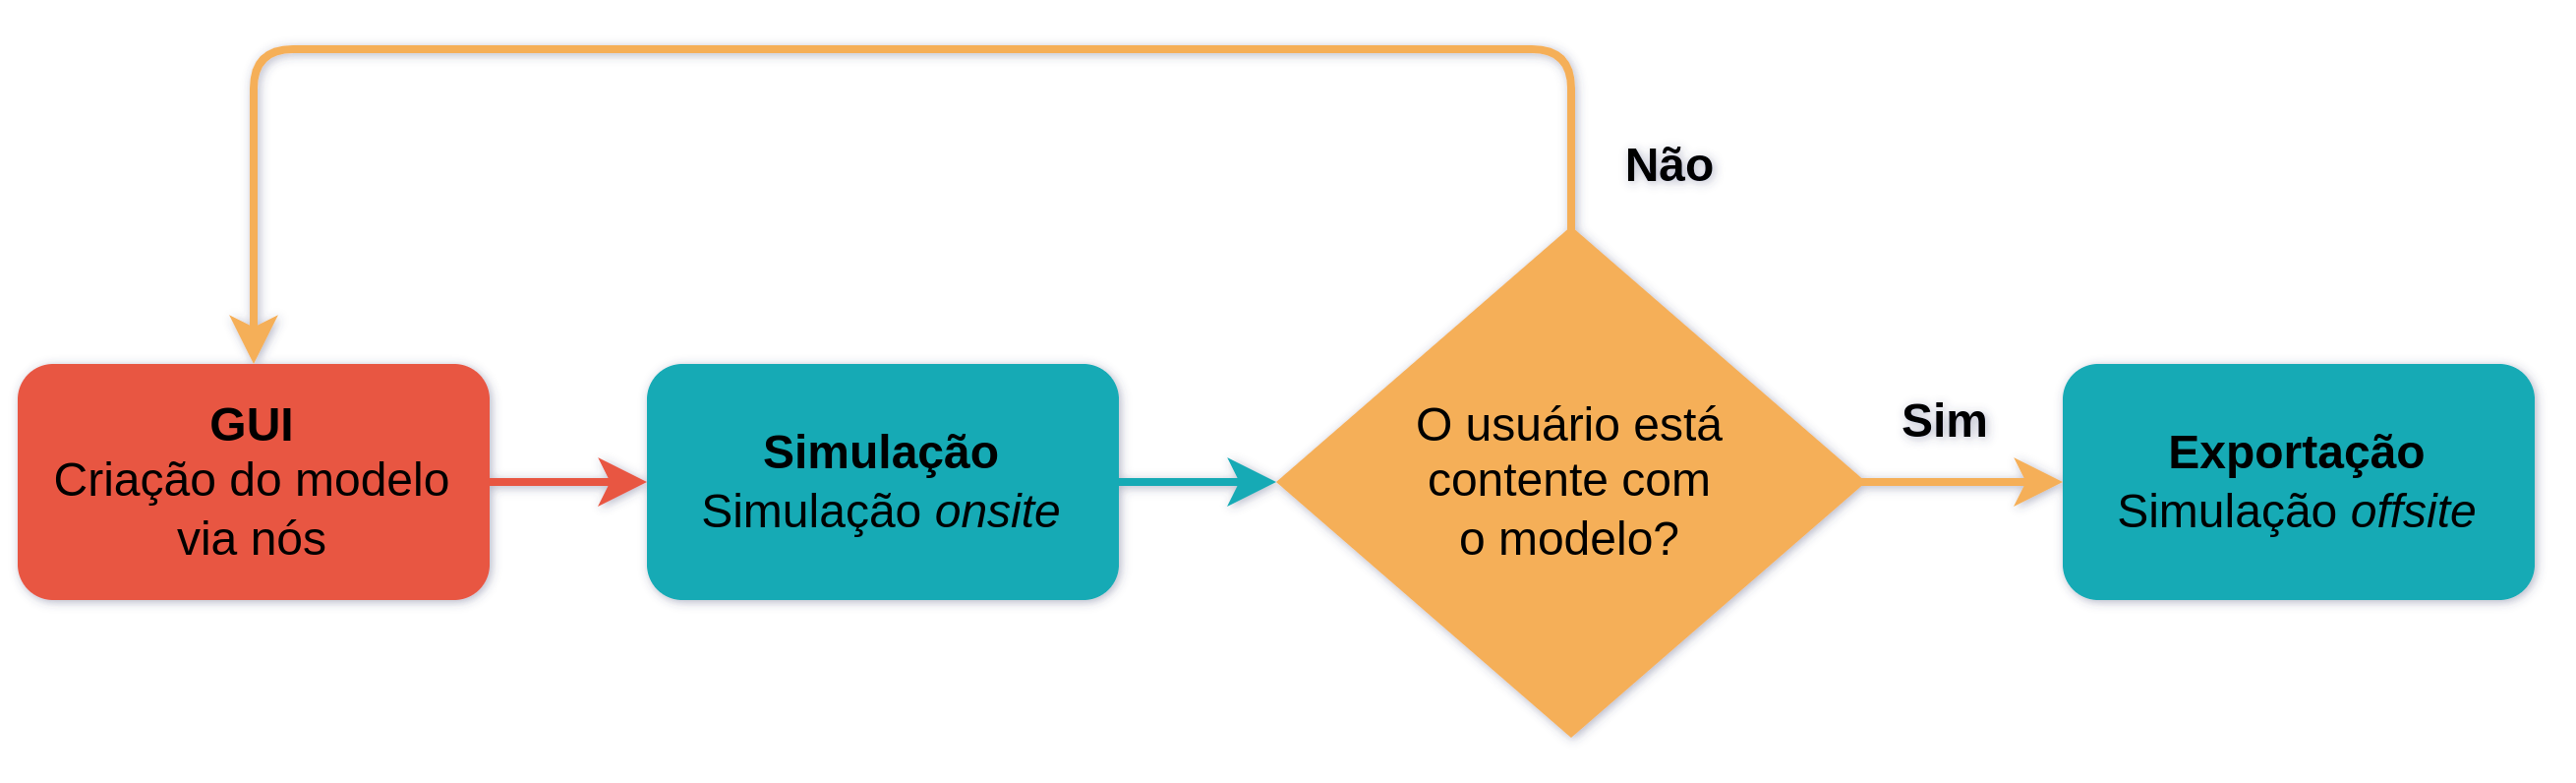
\includegraphics[width=\textwidth, height=\textheight, keepaspectratio=true]{beamerthemesrc/images/ode-designer-fluxograma.png}
%         \caption{Fluxograma da experiência do usuário.}
%     \end{figure}
% \end{frame}

% \begin{frame}{Funcionalidades do Software}
%     O software deve entregar as seguintes funcionalidades:
%     \begin{itemize}
%         \item Criação de modelos pela interface gráfica;
%         \item Simulação do modelo e exibição dos resultados na interface;
%         \item Exportação de PDF/Imagens com os resultados das simulações;
%         \item Exportação de código equivalente ao modelo implementado;
%     \end{itemize}
% \end{frame}

% \subsection{Interface Gráfica}

% \begin{sidepic}{beamerthemesrc/images/ode-designer-gui-exemplo}{Representação do Modelo}
%     \begin{itemize}
%         \item O software necessita de uma interface simples de ser usada;
%             \begin{itemize}
%                 \item Mas também deve naturalmente relembrar uma EDO;
%             \end{itemize}
%         \item Após diversas iterações, chegamos numa interface baseada em programação visual;
%             \begin{itemize}
%                 \item Estas interfaces existem desde 1963, mas tiveram uma renascença com o avanço dos computadores e a necessidade de softwares de edição de imagem/áudio/vídeo;
%             \end{itemize}
%     \end{itemize}
% \end{sidepic}

% \begin{frame}{Fluxo de passagem de informações na interface}
%     \begin{figure}
%         \centering
%         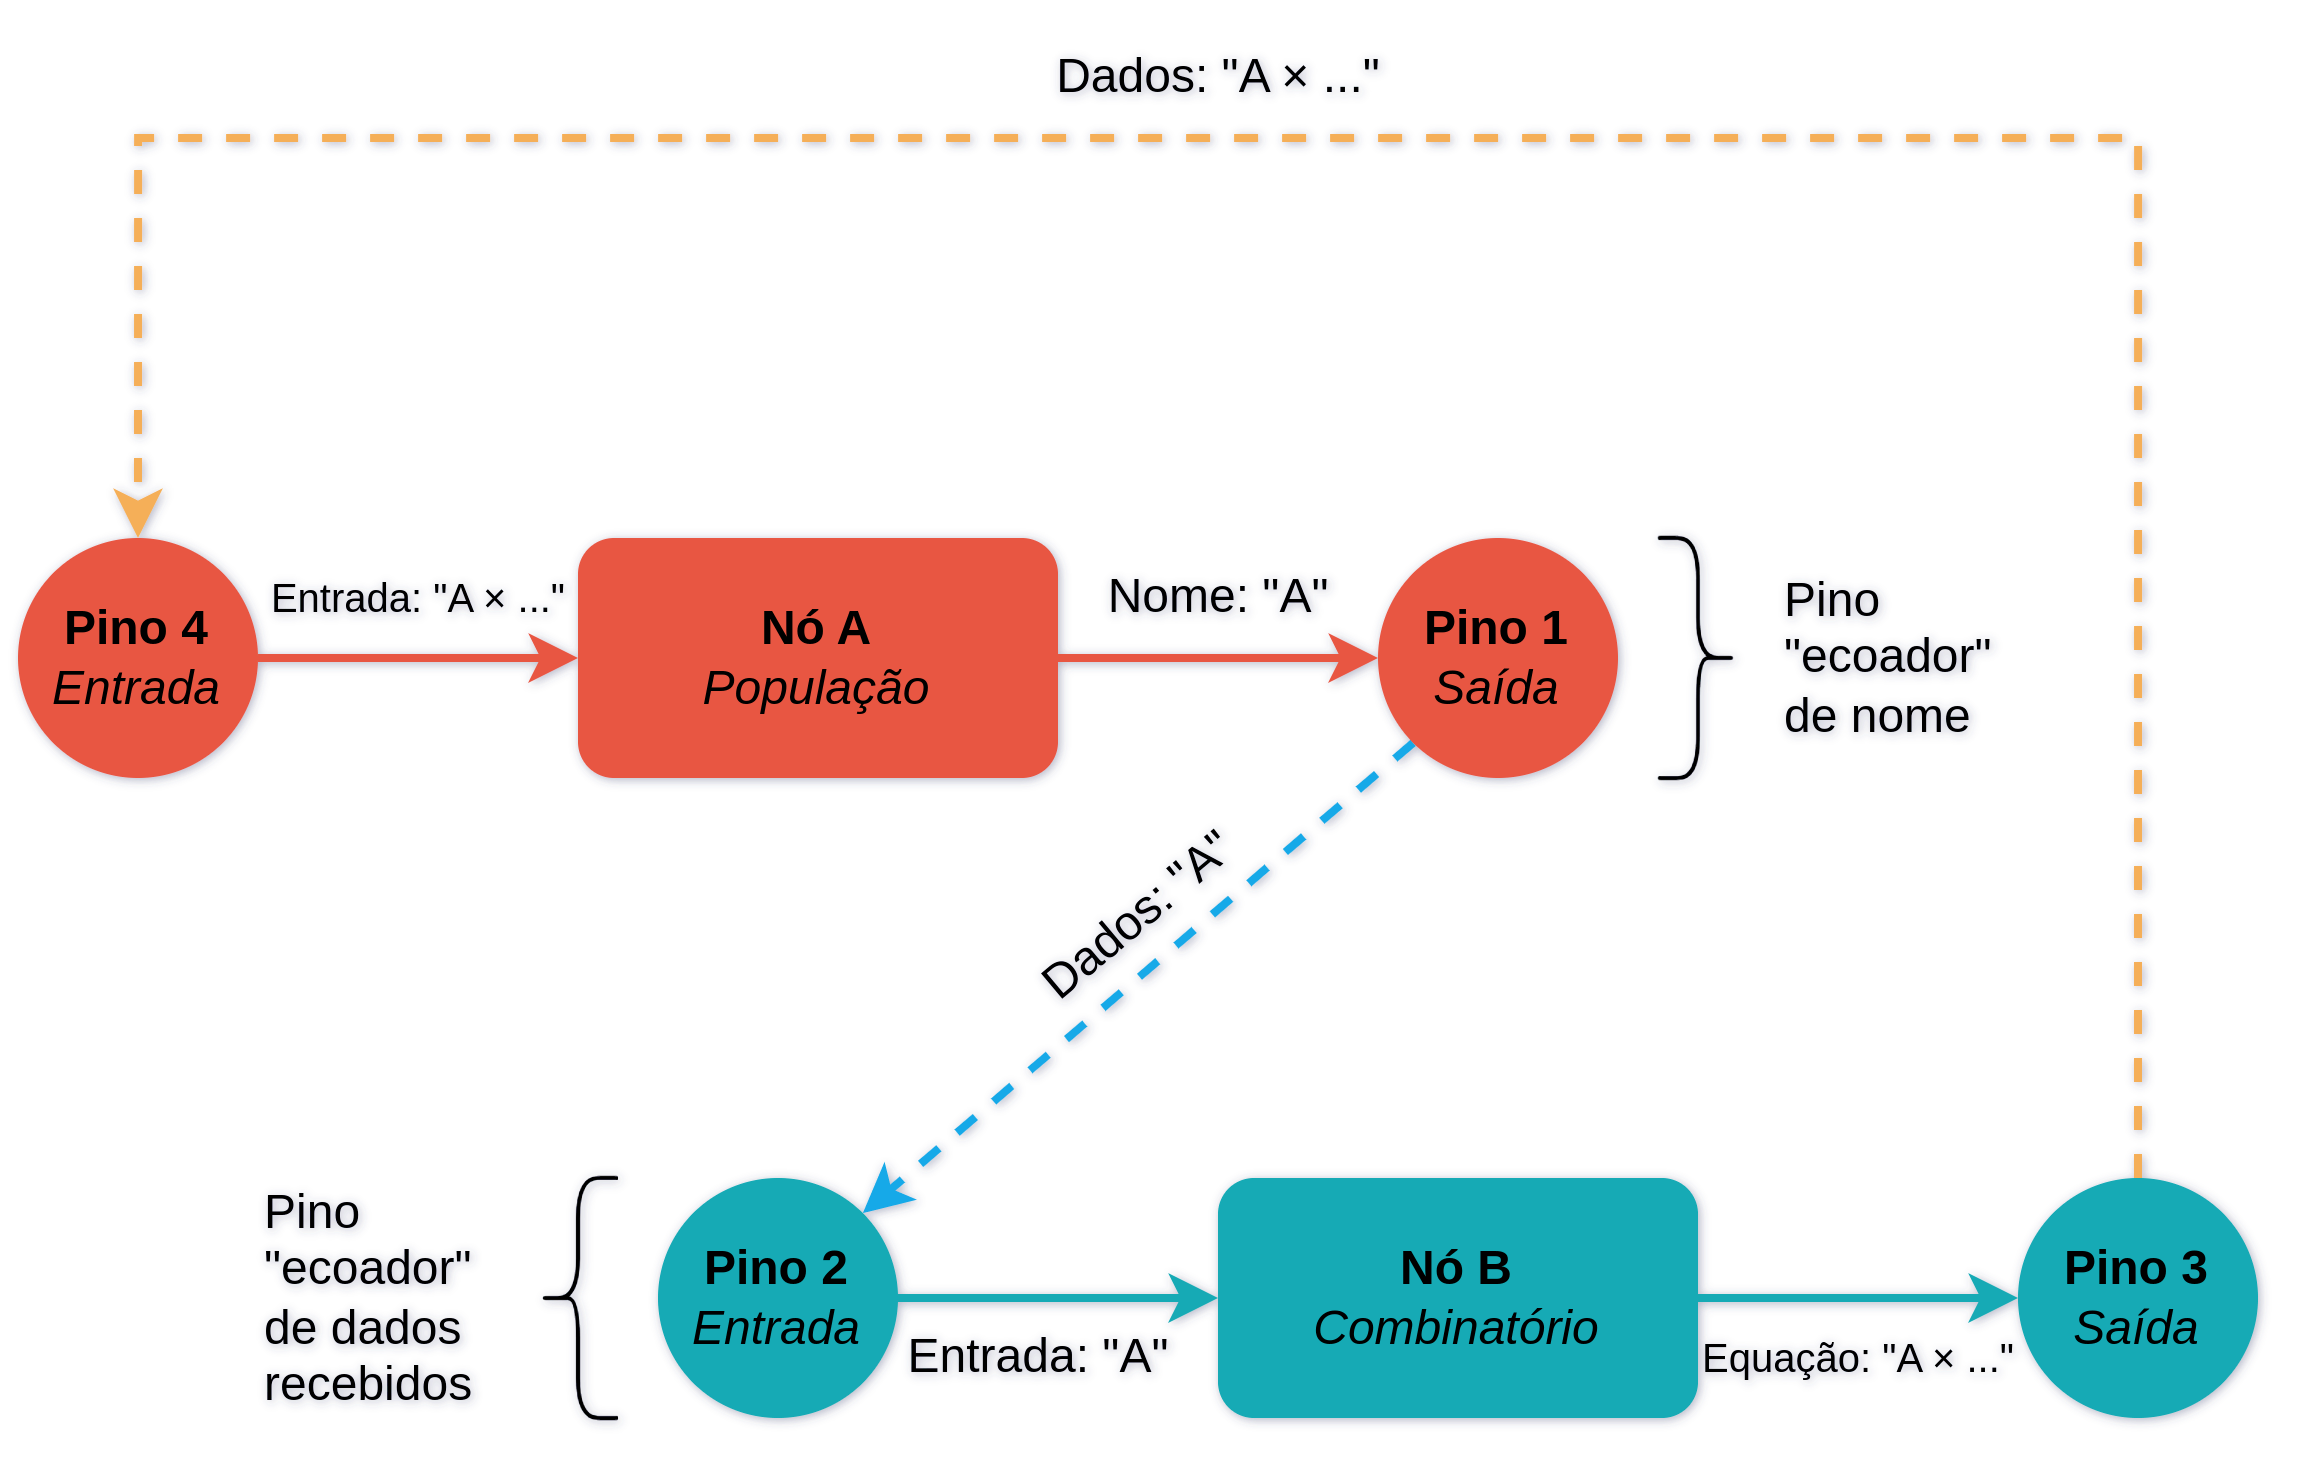
\includegraphics[width=\textwidth, height=\textheight, keepaspectratio=true]{beamerthemesrc/images/fluxo-dados-gui.png}
%         \caption{Relações entre nós e pinos.}
%     \end{figure}
% \end{frame}

% \subsection{Representação Intermediária}

% \begin{chapter}[beamerthemesrc/assets/background_negative]{}{Representação Intermediária}
% \end{chapter}

% \begin{frame}{Representação Intermediária}
%     \begin{itemize}
%         \item Com o objetivo de realizar tantas transformações, torna-se necessário a utilização de uma Representação Intermediária (RI);

%         \item Inspirados nas arquiteturas de compiladores modernos (GCC, baseados em LLVM), separamos a estrutura em back-end e front-end;

%         \item Essa abordagem garante o desacoplamento entre estrutura e produtos finais;
%     \end{itemize}

%     \begin{figure}
%         \centering
%         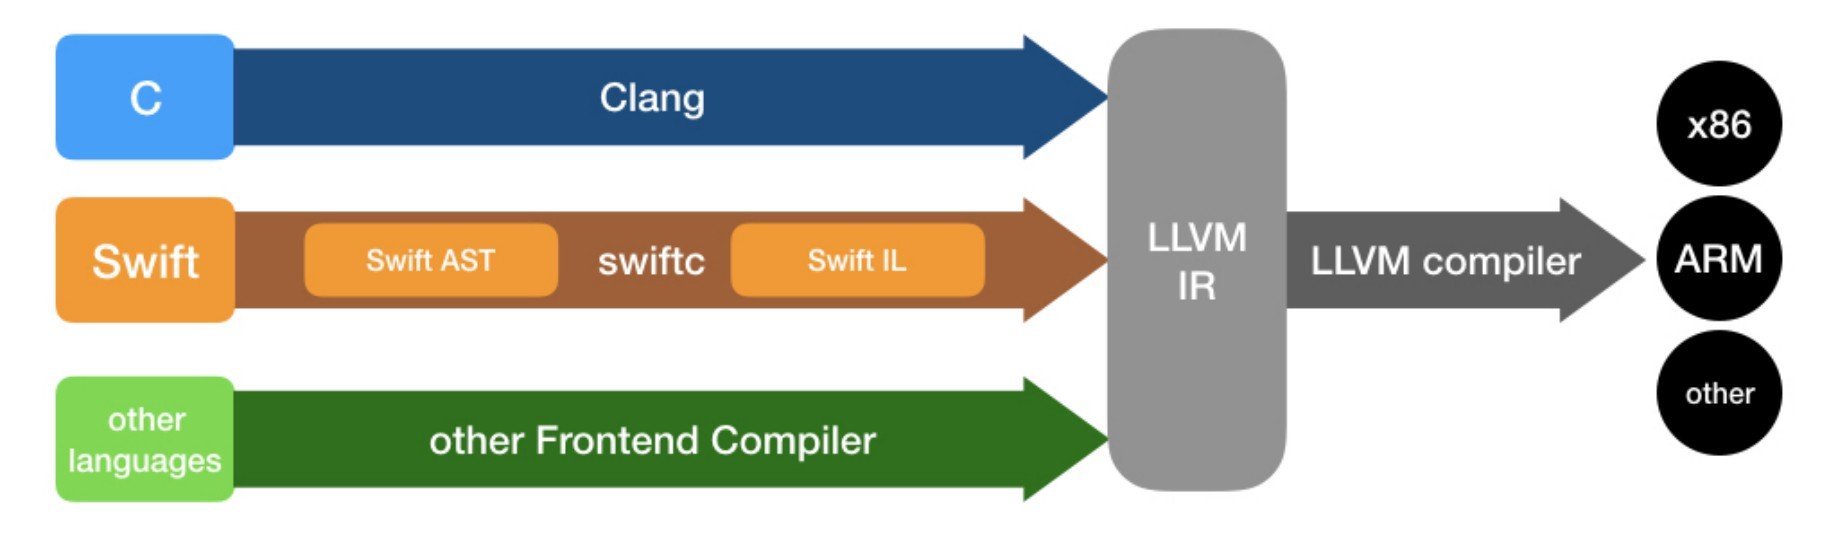
\includegraphics[height=\textheight, width=\textwidth, keepaspectratio=true]{beamerthemesrc/images/llvm-ir.png}
%         \caption{Exemplo de RI: LLVM-IR.}
%     \end{figure}
% \end{frame}

% \begin{frame}[fragile]{RI — Serde: Conversões automatizadas para JSON}
%     \begin{columns}
%         \begin{column}{.55\textwidth}
%             \begin{block}{Rust}
%                 \begin{lstlisting}[language=Rust]
% #[derive(Serialize, Deserialize)]
% struct Person {
%     name: String,
%     age: u8,
%     phones: Vec<String>,
%     address: Address,
% }
% #[derive(Serialize, Deserialize)]
% struct Address {
%     street: String,
%     city: String,
% }
%                 \end{lstlisting}
%             \end{block}
%         \end{column}

%         \begin{column}{.45\textwidth}
%             \begin{block}{JSON}
%                 \begin{lstlisting}[language=json, tabsize=2]
% {
%   "name": "John Doe",
%   "age": 43,
%   "address": {
%     "street": "1st St.",
%     "city": "London"
%   },
%   "phones": [
%     "+44 1234567",
%     "+44 2345678"
%   ]
% }
%                 \end{lstlisting}
%             \end{block}
%         \end{column}
%     \end{columns}
% \end{frame}

% \begin{frame}[fragile]{RI — \textit{Templates}}

%     \begin{itemize}
%         \item \texttt{Structs} \textit{serializáveis} podem ser usadas diretamente em \textit{templates};
%         \item Suponha a variável \texttt{people: Vec<Person>}:
%     \end{itemize}

%     \begin{block}{minijinja}
%         \begin{lstlisting}[language=jinja2]
% 
%     {{ person.name }}, {{ person.age }} anos.
%     Contato: 
%       {{ phone_nb }}
%       , 
%     
% 
%         \end{lstlisting}
%     \end{block}
% \end{frame}

\section{Aplicações do software}
\begin{frame}{Modelo SIRS}
    O modelo SIRS divide a população em indivíduos suscetíveis ($S$) à doença, infectados ($I$) e recuperados ($R$).
    
    Uma parte da população de suscetíveis pode se infectar (termo $\beta.S.I$). Os indivíduos infectados podem se recuperar com uma determinada probabilidade (termo $\alpha.I$) e os indivíduos recuperados podem voltar a ser suscetíveis à doença (termo $\gamma.R$). 
    
    \begin{equation}\label{eq:sirs}
        \begin{array}{lr}
        \frac{dS}{dt} = -\beta.S.I + \gamma.R
        \\
        \\
        \frac{dI}{dt} = \beta.S.I - \alpha.I
        \\
        \\ 
        \frac{dR}{dt} = \alpha.I - \gamma.R
        \end{array}
    \end{equation}
\end{frame}

\begin{frame}{Modelo SIRS - Representação no Software}
    \begin{figure}
        \centering
        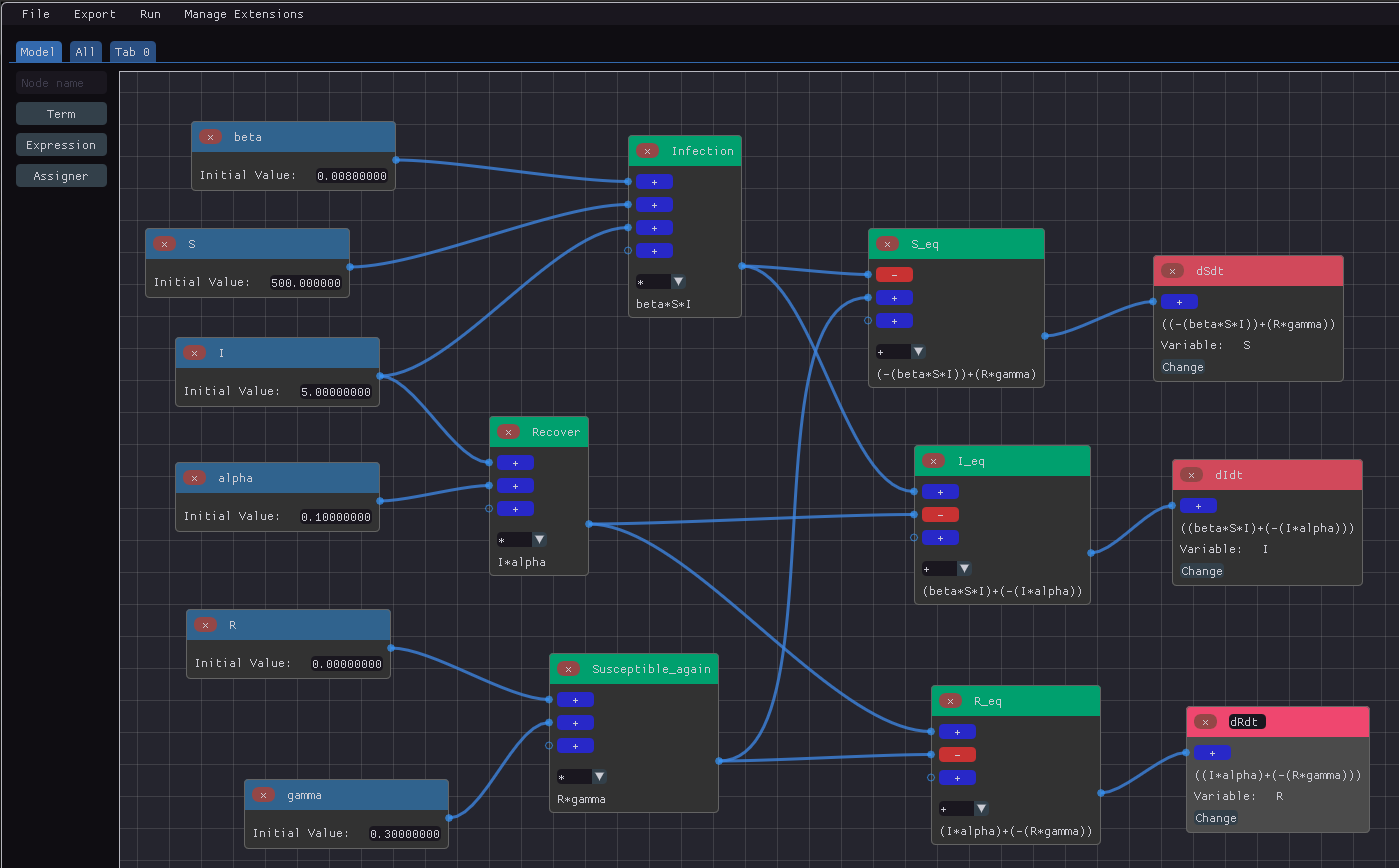
\includegraphics[height=\textheight]{contents/imgs/modelos/sirs.png}
    \end{figure}
\end{frame}

\begin{frame}{Modelo SIRS - Resultados}
    \begin{columns}
        \begin{column}{.2\textwidth}
            \[
            \begin{array}{llr}
                S_0 & = & 500\\
                I_0 & = & 5\\
                R_0 & = & 0\\
                \alpha & = & 0.1\\
                \beta & = & 0.008\\
                \gamma & = & 0.3\\
                \end{array}
            \]
        \end{column}
        \begin{column}{.8\textwidth}
            \begin{figure}
                \centering
                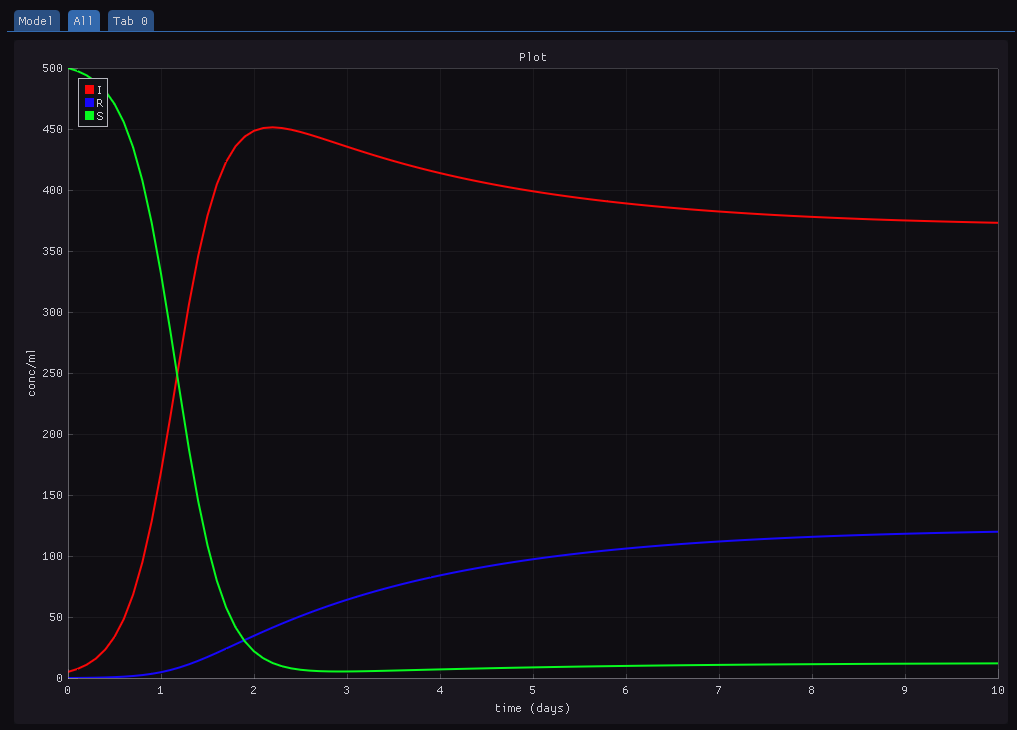
\includegraphics[height=\textheight]{contents/imgs/modelos/resultado-sirs.png}
            \end{figure}
        \end{column}
    \end{columns}
\end{frame}

\section{Conclusões e trabalhos futuros}
\begin{frame}{Conclusões}
    \begin{itemize}
        \item Neste trabalho, foi desenvolvido um software para automatizar a implementação e simulação de modelos computacionais baseados em EDOs.
        \item A construção das equações do modelo matemático é auxiliada pela representação visual que foi criada permitindo que o usuário acompanhe a construção de todas as expressões e como elas estão sendo combinadas para formar o sistema de EDOs.
        \item Através da GUI, é possível ver as entradas e operações de cada expressão, os sinais de cada entrada, quais expressões fazem parte de uma determinada EDO, entre outras coisas. 
    \end{itemize}
\end{frame}

\begin{frame}{Conclusões}
    \begin{itemize}
        \item Como limitações do trabalho, destaca-se: 
        \begin{itemize}
            \item Torna-se mais difícil entender um modelo complexo com muitos nós e ligações. 
            \item Não foi realizada uma avaliação de usabilidade do software. 
        \end{itemize}
    \end{itemize}
\end{frame}

\begin{frame}{Trabalhos futuros}
    \begin{itemize}
        \item Como trabalhos futuros, destaca-se: 
        \begin{itemize}
            \item Geração de código e simulação de modelos estocásticos;
            \note[item]{Modelos estocásticos: utilizando o algoritmo de Gillespie, o mesmo editor de nós e um novo template para a simulação}
            \item Ajustes de parâmetros; 
            \note[item]{Ajustes de parâmetros: fornecendo recursos para o carregamento de dados experimentais, escolha dos parâmetros a serem ajustados e plotagens comparativas}
            \item Análise de sensibilidade de parâmetros;
            \item Geração de código e simulação de Equações Diferenciais Parciais (EDPs);
            \item Desenvolvimento de uma versão Web do software.
            \note[item]{Web: Rust e as tecnologias usadas na interface gráfica possuem suporte nativo à web (via WebAssebmly). Existem distribuições de Python suportadas no navegador, mas uma solução poderia envolver a execução das simulações do lado do servidor ao invés do cliente.}
        \end{itemize}
    \end{itemize}
\end{frame}

\backmatter
\end{document}
